\begin{center}
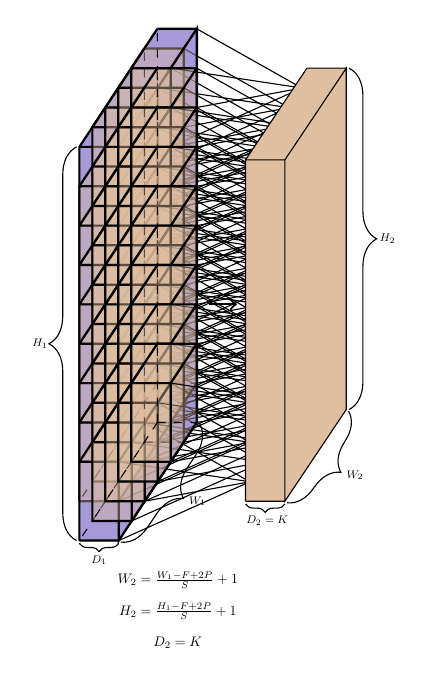
\begin{tikzpicture}[scale=.5, transform shape]
\def\h{10}
\def\w{2}
\def\d{3}
\coordinate (A) at (0,0);
\coordinate (B) at (0,\h);
\coordinate (C) at (\w,\h+\d);
\coordinate (D) at (\w,\d);


\coordinate (A1) at (0+1,0);
\coordinate (B1) at (0+1,\h);
\coordinate (C1) at (\w+1,\h+\d);
\coordinate (D1) at (\w+1,\d);

\fill [draw=none, fill=blue!50] (A) -- (B) -- (C) -- (C1) -- (D1) -- (A1) -- cycle;
\draw (A) -- (B) -- (C) (A) -- (A1) (B) -- (B1) (C) -- (C1) (A1) -- (B1) -- (C1) -- (D1) -- cycle;

\draw [decorate,decoration={brace,amplitude=10pt,raise=1pt},xshift=0pt,yshift=0pt] (A) -- (B) node [black,midway,xshift=-1cm] {\footnotesize $H_1$};

\draw [decorate,decoration={brace,amplitude=3pt,raise=1pt},xshift=-4pt,yshift=0pt] (A1) -- (A) node [black,midway,yshift=-0.5cm] {\footnotesize $D_1$};

\draw [decorate,decoration={brace,amplitude=10pt,mirror,raise=1pt},xshift=0pt,yshift=0pt] (A1) -- (D1) node [black,midway,xshift=1cm,yshift=-0.5cm] {\footnotesize $W_1$};

\def\ha{2}
\def\wa{0.66}
\def\sa{1}
\def\wb{0.33}%shift
\def\sb{0.5}%shift
\def\hc{0.66}%next layer box
\def\wc{0.22}%next layer box size
\def\sc{0.33}
\def\xm{4} %distance of next box
\def\xmv{0.22}
\def\ymv{1}
\def\wid{1}


%layer1 feature map coordinates
\coordinate (A6) at (0+\xm+\xmv,0+\ymv);
\coordinate (B6) at (0+\xm+\xmv,\h-\sc);
\coordinate (C6) at (\w+\xm-\xmv,\h+\d-\ymv);
\coordinate (D6) at (\w+\xm-\xmv,\d+\sc);

\coordinate (A7) at (0+1+\xm+\xmv,0+\ymv);
\coordinate (B7) at (0+1+\xm+\xmv,\h-\sc);
\coordinate (C7) at (\w+1+\xm-\xmv,\h+\d-\ymv);
\coordinate (D7) at (\w+1+\xm-\xmv,\d+\sc);

\fill [draw=none, fill=brown!50] (A6) -- (B6) -- (C6) --  (D6) -- cycle;	


\onslide<1>{
\def\xz{4}
\def\yz{4}
		\coordinate (A2) at (0+\xz*\wb,0+\yz+\xz*\sb);
		\coordinate (B2) at (0+\xz*\wb,\ha+\yz+\xz*\sb);
		\coordinate (C2) at (\wa+\xz*\wb,\ha+\sa+\yz+\xz*\sb);
		\coordinate (D2) at (\wa+\xz*\wb,\sa+\yz+\xz*\sb);
		
		\coordinate (A3) at (0+1+\xz*\wb,0+\yz+\xz*\sb);
		\coordinate (B3) at (0+1+\xz*\wb,\ha+\yz+\xz*\sb);
		\coordinate (C3) at (\wa+1+\xz*\wb,\ha+\sa+\yz+\xz*\sb);
		\coordinate (D3) at (\wa+1+\xz*\wb,\sa+\yz+\xz*\sb);
		
		
		\fill [draw=none, fill=brown!50, fill opacity=0.4] (A2) -- (B2) -- (C2) -- (C3) -- (D3) -- (A3) -- cycle; 
			
		\draw[thick] (A2) -- (B2) -- (C2) (A2) -- (A3) (B2) -- (B3) (C2) -- (C3) (A3) -- (B3) -- (C3) -- (D3) -- cycle;
		\draw[dashed] (D2) -- (A2) (D2) -- (C2) (D2) -- (D3);
		
		\node[] (input1) at (0+0.5+\xz*\wb,0+\yz+\xz*\sb-0.5) {\footnotesize{ \textbf{filter}}};
}		
		


\foreach \y [count=\yi from 0] in {8,7,6,5,4,3,2,1,0}{
	\foreach \x [count=\xi from \yi*5+2] in {0,1,2,3,4}{
		\ifthenelse{\xi<46}{		
		%\onslide<\xi>{	
		%kernel coordinates
		\coordinate (A2) at (0+\x*\wb,0+\y+\x*\sb);
		\coordinate (B2) at (0+\x*\wb,\ha+\y+\x*\sb);
		\coordinate (C2) at (\wa+\x*\wb,\ha+\sa+\y+\x*\sb);
		\coordinate (D2) at (\wa+\x*\wb,\sa+\y+\x*\sb);
		
		\coordinate (A3) at (0+1+\x*\wb,0+\y+\x*\sb);
		\coordinate (B3) at (0+1+\x*\wb,\ha+\y+\x*\sb);
		\coordinate (C3) at (\wa+1+\x*\wb,\ha+\sa+\y+\x*\sb);
		\coordinate (D3) at (\wa+1+\x*\wb,\sa+\y+\x*\sb);
		
		
		%\fill [draw=none, fill=brown!50, fill opacity=0.4] (A2) -- (B2) -- (C2) -- (C3) -- (D3) -- (A3) -- cycle; 
			
		%\draw[thick] (A2) -- (B2) -- (C2) (A2) -- (A3) (B2) -- (B3) (C2) -- (C3) (A3) -- (B3) -- (C3) -- (D3) -- cycle;
		%\draw[dashed] (D2) -- (A2) (D2) -- (C2) (D2) -- (D3);

		%feature map 1, points
		\coordinate (A4) at (0+\x*\wb+\xm+\xmv,0+\y+\x*\sb+\ymv);
		\coordinate (B4) at (0+\x*\wb+\xm+\xmv,\hc+\y+\x*\sb+\ymv);
		\coordinate (C4) at (\wc+\x*\wb+\xm+\xmv,\hc+\sc+\y+\x*\sb+\ymv);
		\coordinate (D4) at (\wc+\x*\wb+\xm+\xmv,\sc+\y+\x*\sb+\ymv);
		\coordinate (ABCD4) at (\wc*0.5+\x*\wb+\xm+\xmv,\y+\x*\sb+\ymv+\hc*0.5+\sc*0.5);
		%\draw (A3) -- (ABCD4);
		%\draw (B3) -- (ABCD4);
		%\draw (C3) -- (ABCD4);
		%\draw (D3) -- (ABCD4);
		
		%}
		%\onslide<\xi->{
			\fill[brown] (ABCD4) ellipse (0.1 and 0.2);		
		%}
		}{
		%\ifthenelse{\xi > 7 \AND \xi < 40}{
		%\onslide<8->{
		\coordinate (A4) at (0+\x*\wb+\xm+\xmv,0+\y+\x*\sb+\ymv);
		\coordinate (B4) at (0+\x*\wb+\xm+\xmv,\hc+\y+\x*\sb+\ymv);
		\coordinate (C4) at (\wc+\x*\wb+\xm+\xmv,\hc+\sc+\y+\x*\sb+\ymv);
		\coordinate (D4) at (\wc+\x*\wb+\xm+\xmv,\sc+\y+\x*\sb+\ymv);
		\coordinate (ABCD4) at (\wc*0.5+\x*\wb+\xm+\xmv,\y+\x*\sb+\ymv+\hc*0.5+\sc*0.5);
		
		%\fill[brown] (ABCD4) ellipse (0.1 and 0.2);
		%}
		%}{
		\pgfmathparse{int(2)}
	 	\onslide<\pgfmathresult>{
		%kernel coordinates
		\coordinate (A2) at (0+\x*\wb,0+\y+\x*\sb);
		\coordinate (B2) at (0+\x*\wb,\ha+\y+\x*\sb);
		\coordinate (C2) at (\wa+\x*\wb,\ha+\sa+\y+\x*\sb);
		\coordinate (D2) at (\wa+\x*\wb,\sa+\y+\x*\sb);
		
		\coordinate (A3) at (0+1+\x*\wb,0+\y+\x*\sb);
		\coordinate (B3) at (0+1+\x*\wb,\ha+\y+\x*\sb);
		\coordinate (C3) at (\wa+1+\x*\wb,\ha+\sa+\y+\x*\sb);
		\coordinate (D3) at (\wa+1+\x*\wb,\sa+\y+\x*\sb);
		
		
		\fill [draw=none, fill=brown!50, fill opacity=0.4] (A2) -- (B2) -- (C2) -- (C3) -- (D3) -- (A3) -- cycle; 
			
		\draw[thick] (A2) -- (B2) -- (C2) (A2) -- (A3) (B2) -- (B3) (C2) -- (C3) (A3) -- (B3) -- (C3) -- (D3) -- cycle;
		\draw[dashed] (D2) -- (A2) (D2) -- (C2) (D2) -- (D3);

		%feature map 1, points
		\coordinate (A4) at (0+\x*\wb+\xm+\xmv,0+\y+\x*\sb+\ymv);
		\coordinate (B4) at (0+\x*\wb+\xm+\xmv,\hc+\y+\x*\sb+\ymv);
		\coordinate (C4) at (\wc+\x*\wb+\xm+\xmv,\hc+\sc+\y+\x*\sb+\ymv);
		\coordinate (D4) at (\wc+\x*\wb+\xm+\xmv,\sc+\y+\x*\sb+\ymv);
		\coordinate (ABCD4) at (\wc*0.5+\x*\wb+\xm+\xmv,\y+\x*\sb+\ymv+\hc*0.5+\sc*0.5);
		\draw (A3) -- (ABCD4);
		\draw (B3) -- (ABCD4);
		\draw (C3) -- (ABCD4);
		\draw (D3) -- (ABCD4);
		
		}
		\onslide<\pgfmathresult->{
			\fill[brown] (ABCD4) ellipse (0.1 and 0.2);		
		}
		%};
		};
	}
	
}

\onslide<3->{
		\draw[thick,->] (3.3,6) -- (4,6);

		\fill [draw=none, fill=brown!50] (A6) -- (B6) -- (C6) -- (C7) -- (D7) -- (A7) -- cycle;
		\draw [black] (A6) -- (B6) -- (C6) (A6) -- (A7) (B6) -- (B7) (C6) -- (C7) (A7) -- (B7) -- (C7) -- (D7) -- cycle;
		
\draw [decorate,decoration={brace,amplitude=10pt,raise=1pt},xshift=0pt,yshift=0pt] (C7) -- (D7) node [midway,xshift=1cm] { \footnotesize{ $H_2$}};

\draw [decorate,decoration={brace,amplitude=3pt,raise=1pt},xshift=-4pt,yshift=0pt] (A7) -- (A6) node [black,midway,yshift=-0.5cm] { \footnotesize{ $D_2 = K$}};

\draw [decorate,decoration={brace,amplitude=10pt,mirror,raise=1pt},xshift=0pt,yshift=0pt] (A7) -- (D7) node [black,midway,xshift=1cm,yshift=-0.5cm] { \footnotesize{$W_2$}};

\node (m1) at (2.5,-1) {$W_2 = \frac{W_1-F+2P}{S}+1$};
\node (m1) at (2.5,-1.8) {$H_2 = \frac{H_1-F+2P}{S}+1$};
\node (m1) at (2.5,-2.6) {$D_2 = K$};
}
\end{tikzpicture}
\end{center}